% fig_hif_margin.tex — TPR vs scaled fault current for 87L and 87B zones
% Solid blue = conventional; dashed red = SAMBP
% Shows 87L sensitivity degradation, 87B perfect detection
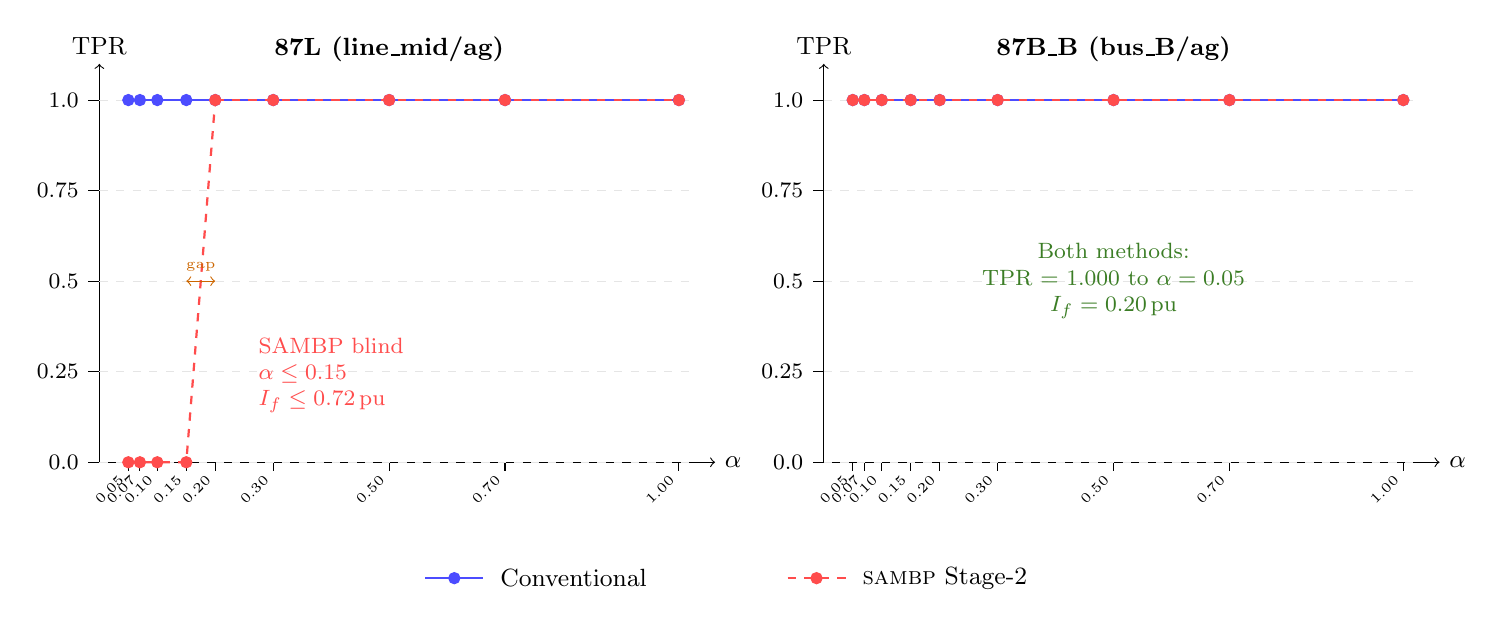
\begin{tikzpicture}[scale=0.92]

% Shared axis setup
% X axis: I_f scaled [pu] from 0 to 10, log-ish but linear for clarity
% Use linear x mapped from alpha × I_f_nom

%-------------------------------------------------------------------
% Left plot: 87L ag (line_mid/ag — I_f_nom=4.8 pu)
%   alpha:  1.00  0.70  0.50  0.30  0.20  0.15  0.10  0.07  0.05
%   I_f:    4.8   3.36  2.40  1.44  0.96  0.72  0.48  0.336 0.24
%   conv:   1     1     1     1     1     1     1     1     1
%   sambp:  1     1     1     1     1     0     0     0     0
%
% Normalised X: I_f / I_f_nom, so X ∈ [0.05, 1] → map to 0..8 cm

\begin{scope}[xshift=0cm]

% Axes
\draw[->] (0,0)--(8.5,0) node[right,font=\small]{$\alpha$};
\draw[->] (0,0)--(0,5.5) node[above,font=\small]{TPR};

% X ticks (alpha values)
\foreach \a/\lbl in {8.0/1.00, 5.6/0.70, 4.0/0.50, 2.4/0.30, 1.6/0.20, 1.2/0.15, 0.8/0.10, 0.56/0.07, 0.4/0.05}{
    \draw (\a,0)--(\a,-0.12) node[below,font=\tiny,rotate=45,anchor=east]{\lbl};
}
% Y ticks
\foreach \y/\v in {0/0.0,1.25/0.25,2.5/0.5,3.75/0.75,5.0/1.0}{
    \draw (0,\y)--(-0.15,\y) node[left,font=\footnotesize]{\v};
    \draw[gray!20,dashed](0,\y)--(8.2,\y);
}

% Conv line (always 1.000)
\draw[blue!70,thick]
  (0.4,5.0)--(0.56,5.0)--(0.8,5.0)--(1.2,5.0)--(1.6,5.0)
  --(2.4,5.0)--(4.0,5.0)--(5.6,5.0)--(8.0,5.0);
\foreach \x in {0.4,0.56,0.8,1.2,1.6,2.4,4.0,5.6,8.0}{
    \filldraw[blue!70] (\x,5.0) circle(2.2pt);}

% SAMBP line (drops to 0 at alpha<=0.15)
%  alpha: 1.00→5.0, 0.70→5.0, 0.50→5.0, 0.30→5.0, 0.20→5.0, 0.15→0.0, ...
\draw[red!70,thick,dashed]
  (1.6,5.0)--(2.4,5.0)--(4.0,5.0)--(5.6,5.0)--(8.0,5.0);
\draw[red!70,thick,dashed]
  (0.4,0.0)--(0.56,0.0)--(0.8,0.0)--(1.2,0.0)--(1.6,5.0);
\foreach \x/\y in {8.0/5.0,5.6/5.0,4.0/5.0,2.4/5.0,1.6/5.0,1.2/0.0,0.8/0.0,0.56/0.0,0.4/0.0}{
    \filldraw[red!70] (\x,\y) circle(2.2pt);}

% Threshold arrow
\draw[<->,orange!80!black,thin] (1.2,2.5)--(1.6,2.5)
  node[midway,above,font=\tiny]{gap};

% Label
\node[font=\small\bfseries] at (4.0,5.7) {87L (line\_mid/ag)};
\node[font=\footnotesize,align=left,text=red!70] at (3.2,1.2)
  {SAMBP blind\\$\alpha \leq 0.15$\\$I_f \leq 0.72$\,pu};

\end{scope}

%-------------------------------------------------------------------
% Right plot: 87B ag (bus_B/ag — I_f_nom=4.0 pu)
%   alpha:   1.00  0.70  0.50  0.30  0.20  0.15  0.10  0.07  0.05
%   I_f:     4.0   2.8   2.0   1.2   0.8   0.6   0.4   0.28  0.20
%   conv:    1     1     1     1     1     1     1     1     1
%   sambp:   1     1     1     1     1     1     1     1     1

\begin{scope}[xshift=10cm]

\draw[->] (0,0)--(8.5,0) node[right,font=\small]{$\alpha$};
\draw[->] (0,0)--(0,5.5) node[above,font=\small]{TPR};

\foreach \a/\lbl in {8.0/1.00,5.6/0.70,4.0/0.50,2.4/0.30,1.6/0.20,1.2/0.15,0.8/0.10,0.56/0.07,0.4/0.05}{
    \draw (\a,0)--(\a,-0.12) node[below,font=\tiny,rotate=45,anchor=east]{\lbl};
}
\foreach \y/\v in {0/0.0,1.25/0.25,2.5/0.5,3.75/0.75,5.0/1.0}{
    \draw (0,\y)--(-0.15,\y) node[left,font=\footnotesize]{\v};
    \draw[gray!20,dashed](0,\y)--(8.2,\y);
}

% Both lines at 1.000 always
\draw[blue!70,thick]
  (0.4,5.0)--(0.56,5.0)--(0.8,5.0)--(1.2,5.0)--(1.6,5.0)
  --(2.4,5.0)--(4.0,5.0)--(5.6,5.0)--(8.0,5.0);
\foreach \x in {0.4,0.56,0.8,1.2,1.6,2.4,4.0,5.6,8.0}{
    \filldraw[blue!70] (\x,5.0) circle(2.2pt);}

\draw[red!70,thick,dashed]
  (0.4,5.0)--(0.56,5.0)--(0.8,5.0)--(1.2,5.0)--(1.6,5.0)
  --(2.4,5.0)--(4.0,5.0)--(5.6,5.0)--(8.0,5.0);
\foreach \x in {0.4,0.56,0.8,1.2,1.6,2.4,4.0,5.6,8.0}{
    \filldraw[red!70] (\x,5.0) circle(2.2pt);}

\node[font=\small\bfseries] at (4.0,5.7) {87B\_B (bus\_B/ag)};
\node[font=\footnotesize,align=center,text=OliveGreen] at (4.0,2.5)
  {Both methods:\\TPR = 1.000 to $\alpha = 0.05$\\$I_f = 0.20$\,pu};

\end{scope}

% Shared legend
\draw[blue!70,thick] (4.5,-1.6)--(5.3,-1.6);
\filldraw[blue!70] (4.9,-1.6) circle(2.2pt);
\node[right,font=\small] at (5.4,-1.6) {Conventional};
\draw[red!70,thick,dashed] (9.5,-1.6)--(10.3,-1.6);
\filldraw[red!70] (9.9,-1.6) circle(2.2pt);
\node[right,font=\small] at (10.4,-1.6) {\textsc{sambp} Stage-2};

\end{tikzpicture}
